\subsection{Objects in the amber.sieve package}


\begin{figure}[htp]
  \centering
  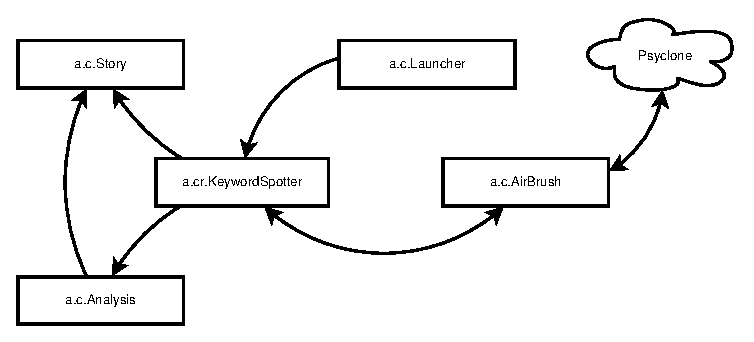
\includegraphics{image/sieve}
  \caption{\label{fig:sieve}Object model of a Sieve module. Arrows
    represent the presence of references to the object where it is pointing to
    in the object where it is pointing from.}
\end{figure}

\classname{KeywordSpotter}

\begin{classmetadata}
  \extends{Sieve}
  \implements{amber.common.AirBrushCallable}
  \function{The KeywordSpotter is configured to detect the presence of certain
            keywords in a story which makes it fit in a certain category or
            subject. In early versions the weights of the subjects will be
            equal. In later versions all weights of all subjects of a story
            must for instance add up to 100\%.  This gives the visualizer more
            freedom to place the story.}
\end{classmetadata}

% \begin{interface}
% \end{interface}


